\documentclass[a4paper,12pt, titlepage]{article}
\usepackage{amssymb,amsthm,amsmath}
\usepackage[finnish]{babel}
\usepackage[T1]{fontenc}
\usepackage[utf8]{inputenc}
\usepackage{graphicx}
\usepackage{hyperref}
\linespread{1.24}
\sloppy

\title{Tietokantasovellus \\ Dokumentaatio}
\author{Andreas Niskanen}
\date{\today}

\begin{document}

\maketitle

\tableofcontents

\newpage

\section{Johdanto}

Kisällikursseilla opiskelijat palauttavat viikoittain harjoitustehtäviä,
joista he voivat ansaita lisäpisteitä kurssisuoritukseen. Tehtäviä on
kahdenlaisia. Tähtitehtävät tarkistetaan, ja niistä saa pisteitä vain
silloin, kun tehtävä on tehty oikein. Tehtäviä saa kuitenkin korjata ja
palauttaa uudelleen. Tähdettömiä tehtäviä ei sen sijaan tarkisteta.\\
Tämä käytäntö vaatii toimiakseen pistekirjanpitojärjestelmän, jonka avulla
ohjaajat voivat kirjata opiskelijan palauttamia tehtäviä ja näiden korjauksia
mahdollisimman sujuvasti. Ohjaajan tulee myös nähdä opiskelijan palauttamat
tehtävät sopivassa muodossa ja muokata näitä tarpeen mukaan.\\
Kurssin opettajan vastuulla on lisätä järjestelmään kursseja ja poistaa
niitä järjestelmästä, sekä lisätä kullekin kurssille harjoitustehtäviä ja
hyväksyä ohjaajia, joilla on oikeudet muokata vain oman kurssin palautuksia.
Lisäksi opettajat tarvitsevat tiettyjä tilastollisia tunnuslukuja (esimerkiksi
palautettujen tehtävien määristä), jotka tulee näkyä kunkin kurssin yhteydessä.\\
Kyseinen pistekirjanpitojärjestelmä toteutetaan tietojenkäsittelytieteen
laitoksen users-palvelimelle käyttäen PostgreSQL-tietokantapalvelinta.
Palvelimen puolella käytetään PHP-ohjelmointikieltä, jonka avulla haetaan
tarvittava data tietokannasta ja vastataan käyttäjän selaimen pyyntöihin.

\newpage

\section{Yleiskuva järjestelmästä}

\subsection{Käyttötapauskaavio}

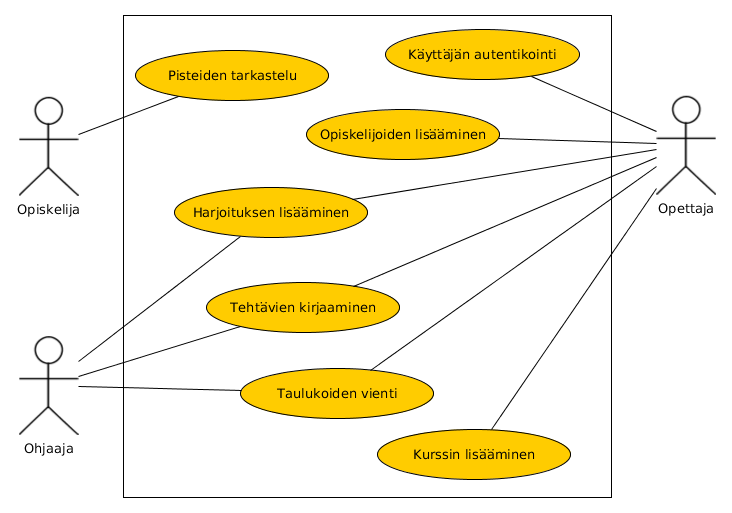
\includegraphics[scale=0.5]{kayttotapauskaavio}

\subsection{Käyttäjäryhmät}

\begin{description}
	\item[Opiskelija] \hfill \\
	Opiskelijalla tarkoitetaan ketä tahansa, joka päätyy kyseisen
	järjestelmän web-sivulle. Kaikki muut käyttäjäryhmät kuuluvat
	myös tähän käyttäjäryhmään.
	\item[Ohjaaja] \hfill \\
	Ohjaaja on järjestelmään rekisteröitynyt käyttäjä, jonka vastuulla
	on oman kurssin palautukset.
	\item[Opettaja] \hfill \\
	Opettaja on järjestelmään rekisteröitynyt käyttäjä, jonka
	vastuulla on omat kurssit.
\end{description}

\subsection{Käyttötapauskuvaukset}

\begin{description}
	\item[Opiskelijan käyttötapaukset] \hfill \\
	\begin{description}
		\item[Pisteiden tarkastelu] \hfill \\
		Opiskelija pystyy järjestelmän etusivulta tarkastamaan
		omat pisteensä valitsemalla kurssin ja syöttämällä
		oman kurssitunnuksensa.
		\item[Muut käyttötapaukset:] rekisteröityminen, kirjautuminen
	\end{description}
	\item[Ohjaajan käyttötapaukset] \hfill \\
	\begin{description}
		\item[Tehtävien kirjaaminen] \hfill \\
		Ohjaajan tehtävänä on kirjata järjestelmään oman kurssin tehtäviä.
		Ohjaajan tulee myös tarvittaessa pystyä katsomaan ja muokkaamaan
		jo kirjattuja opiskelijan harjoituksen tehtäviä.
		\item[Harjoituksen lisääminen] \hfill \\
		Ohjaajan tehtäviin kuuluu myös lisätä omille kursseille harjoituksia
		määrittelemällä tehtävien lukumäärä. Ohjaaja pystyy tarvittaessa
		myös muokkaamaan ja poistamaan harjoituksia.
		\item[Taulukoiden vienti] \hfill \\
		Ohjaaja pystyy tulostamaan järjestelmästä taulukkona tietyn kurssin
		kaikkien opiskelijoiden palautettujen tehtävien lukumäärät, esimerkiksi
		.csv-muodossa.
		\item[Muut käyttötapaukset:] rekisteröityminen, kirjautuminen
	\end{description}
	\item[Opettajan käyttötapaukset] \hfill \\
	\begin{description}
		\item[Käyttäjän autentikointi] \hfill \\
		Kun ohjaaja tai opettaja rekisteröityy järjestelmään,
		opettajan tulee vahvistaa kyseinen käyttäjä.
		\item[Kurssin lisääminen] \hfill \\
		Opettajan tehtäviin kuuluu lisätä järjestelmään omia kursseja.
		Opettaja pystyy tarvittaessa myös muokkaamaan ja poistamaan kursseja.
		\item[Opiskelijoiden lisääminen] \hfill \\
		Opettajan tehtäviin kuuluu myös lisätä omille kursseille opiskelijoita
		kurssitunnuksen mukaan. Opettaja pystyy tarvittaessa myös muokkaamaan
		ja poistamaan opiskelijoita.
		\item[Muut käyttötapaukset:] rekisteröityminen, kirjautuminen,
		tehtävien kirjaaminen, harjoituksen lisääminen, taulukoiden vienti
	\end{description}
\end{description}

\section{Järjestelmän tietosisältö}

\subsection{Käsitekaavio}

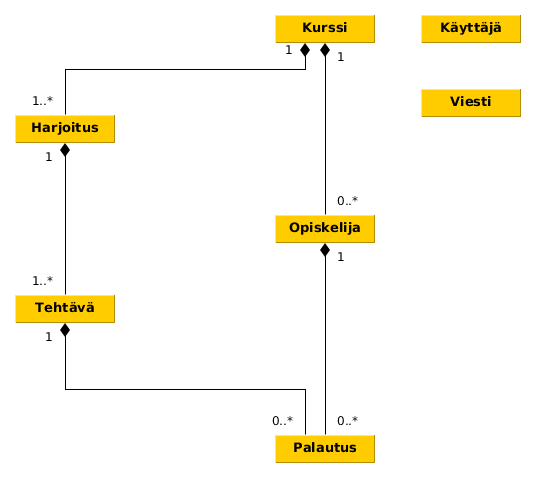
\includegraphics[scale=0.5]{kasitekaavio}

\subsection{Tietokohteet}

\begin{description}
	\item[Tietokohde: Käyttäjä] \hfill \\
	\begin{tabular}{| l | l |}
	\hline
	Attribuutti & Arvojoukko \\ \hline
	Nimi & Merkkijono, max. 50 merkkiä \\ \hline
	Sähköpostiosoite & Merkkijono, max. 50 merkkiä \\ \hline
	Salasana & Merkkijono, max. 60 merkkiä \\ \hline
	On opettaja & Totuusarvo \\ \hline
	\end{tabular}
	\item[Tietokohde: Kurssi] \hfill \\
	\begin{tabular}{| l | l |}
	\hline
	Attribuutti & Arvojoukko \\ \hline
	Nimi & Merkkijono, max. 50 merkkiä \\ \hline
	Lukukausi & Merkkijono, max. 50 merkkiä \\ \hline
	\end{tabular}
	\item[Tietokohde: Opiskelija] \hfill \\
	\begin{tabular}{| l | l |}
	\hline
	Attribuutti & Arvojoukko \\ \hline
	Opiskelijanumero & Merkkijono, max. 50 merkkiä \\ \hline
	Kurssitunnus & Merkkijono, max. 50 merkkiä \\ \hline
	Kurssin id & Kokonaisluku \\ \hline
	\end{tabular}
	\item[Tietokohde: Harjoitus] \hfill \\
	\begin{tabular}{| l | l |}
	\hline
	Attribuutti & Arvojoukko \\ \hline
	Harjoitusnumero & Kokonaisluku \\ \hline
	Tehtävien lukumäärä & Kokonaisluku \\ \hline
	Tähtitehtävien lukumäärä & Kokonaisluku \\ \hline
	Kurssin id & Kokonaisluku \\ \hline
	\end{tabular}
	\item[Tietokohde: Tehtävä] \hfill \\
	\begin{tabular}{| l | l |}
	\hline
	Attribuutti & Arvojoukko \\ \hline
	Tehtävänumero & Kokonaisluku \\ \hline
	On tähtitehtävä & Totuusarvo \\ \hline
	Harjoituksen id & Kokonaisluku \\ \hline
	\end{tabular}
	\item[Tietokohde: Palautus] \hfill \\
	\begin{tabular}{| l | l |}
	\hline
	Attribuutti & Arvojoukko \\ \hline
	Arvosana & 1 merkki \\ \hline
	Tehtävän id & Kokonaisluku \\ \hline
	Opiskelijan id & Kokonaisluku \\ \hline
	\end{tabular}
	\item[Tietokohde: Viesti] \hfill \\
	\begin{tabular}{| l | l |}
	\hline
	Attribuutti & Arvojoukko \\ \hline
	Lähettäjän nimi & Merkkijono \\ \hline
	Lähettäjän sähköpostiosoite & Merkkijono \\ \hline
	Lähettäjän salasana & Merkkijono \\ \hline
	Lähettäjä on opettaja & Totuusarvo \\ \hline
	\end{tabular}
\end{description}

\section{Relaatiotietokantakaavio}

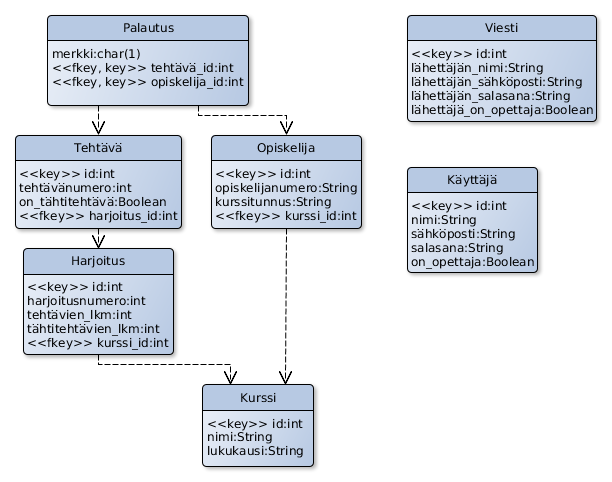
\includegraphics[scale=0.5]{relaatiokaavio}

\section{Järjestelmän yleisrakenne}

Kyseistä tietokantasovellusta tehdessä on noudatettu MVC-mallia.
Mallit, näkymät ja kontrollerit on sijoitettu app-kansion hakemistoihin models, views ja controllers.
Sovellus käyttää istuntoa käyttäjän kirjautumisen havaitsemiseen.

\section{Käyttöliittymä ja järjestelmän komponentit}

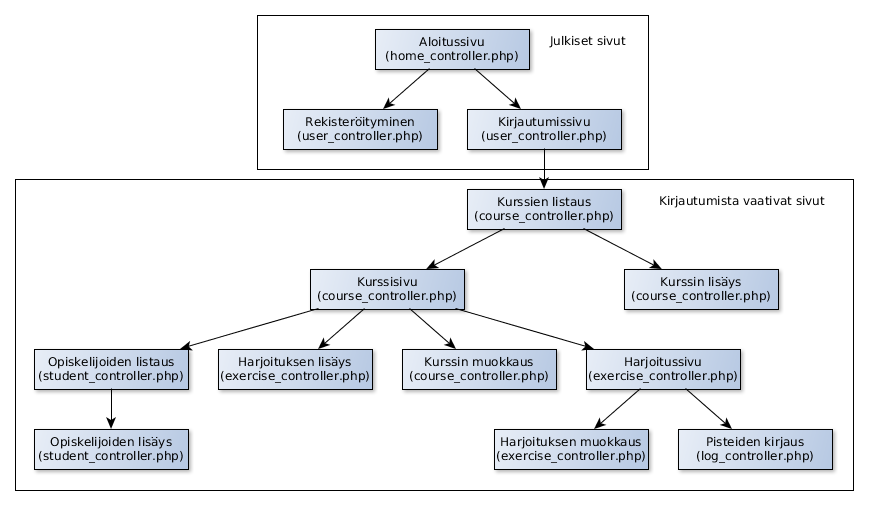
\includegraphics[scale=0.45]{kayttoliittyma}

\section{Asennustiedot}

Asenna sovellus kopioimalla sen tiedostot palvelimen nettiin näkyvään hakemistoon (esim. usersin htdocs-hakemisto).
Asenna sen jälkeen tietokannan yhteystiedot oikeaksi tiedostoon \verb|config/environment.sh|.

\section{Käynnistys- / käyttöohje}

Harjoitustyö on asennettuna osoitteessa \url{http://andreasn.users.cs.helsinki.fi/pkp/}.
Kirjautumista voi kokeilla sähköpostiosoitteella \verb|andreasn@cs.helsinki.fi|
ja salasanalla \verb|asdasd123456|.

\end{document}
